%%%%%%%%%%%%%%%%%%%%%%%%%%%%%%%%%%%%%%%%%%%%%%%%%%%%%%%
% A template for Wiley article submissions.
% Developed by Overleaf. 
%
% Please note that whilst this template provides a 
% preview of the typeset manuscript for submission, it 
% will not necessarily be the final publication layout.
%
% Usage notes:
% The "blind" option will make anonymous all author, affiliation, correspondence and funding information.
% Use "num-refs" option for numerical citation and references style.
% Use "alpha-refs" option for author-year citation and references style.

\documentclass[alpha-refs]{wiley-article}

% Add additional packages here if required
\usepackage{multirow}
\usepackage{gensymb}

% Update article type if known
\papertype{Original Article}
% Include section in journal if known, otherwise delete
%\paperfield{Journal Section}

\title{Should we use ERA5 for statistical precipitation downscaling with analog methods?}

% List abbreviations here, if any. Please note that it is preferred that abbreviations be defined at the first instance they appear in the text, rather than creating an abbreviations list.
\abbrevs{ABC, a black cat; DEF, doesn't ever fret; GHI, goes home immediately.}

% Include full author names and degrees, when required by the journal.
% Use the \authfn to add symbols for additional footnotes and present addresses, if any. Usually start with 1 for notes about author contributions; then continuing with 2 etc if any author has a different present address.
\author[1]{Pascal Horton}

% Include full affiliation details for all authors
\affil[1]{Oeschger Centre for Climate Change Research and Institute of Geography, University of Bern, Bern, Switzerland}

\corraddress{Pascal Horton, Oeschger Centre for Climate Change Research and Institute of Geography, University of Bern, 3012 Bern, Switzerland}
\corremail{pascal.horton@alumni.epfl.ch}

%\presentadd[\authfn{2}]{Department, Institution, City, State or Province, Postal Code, Country}

%\fundinginfo{Funder One, Funder One Department, Grant/Award Number: 123456, 123457 and 123458; Funder Two, Funder Two Department, Grant/Award Number: 123459}

% Include the name of the author that should appear in the running header
\runningauthor{P. Horton}

\begin{document}

\maketitle

\begin{abstract}
This is a generic template designed for use by multiple journals, which includes several options for customization. Please consult the author guidelines for the journal to which you are submitting in order to confirm that your manuscript will comply with the journal's requirements. Please replace this text with your abstract.

% Please include a maximum of seven keywords
\keywords{keyword 1, \emph{keyword 2}, keyword 3, keyword 4, keyword 5, keyword 6, keyword 7}
\end{abstract}

\section{Introduction}

\section{Data and methods}

\subsection{Reanalyses}

The present work aims at comparing ERA5 \citep{Hersbach2019} to other global reanalyses, which characteristics are provided in Table \ref{table:datasets}. The three first reanalyses are surface-input \citep{Fujiwara2017} products that assimilate surface data only, but cover a long period, typically the 20th century. NOAA produced the Twentieth Century Reanalysis \citep[version 2c, 20CR-2c --][]{Compo2011} which only assimilates surface pressure data and uses observed monthly sea-surface temperature and sea-ice distributions as boundary conditions. The European Centre for Medium-Range Weather Forecasts (ECMWF) developed two products using surface input only: ERA-20C \citep{Poli2016} that assimilates marine wind observations and is forced by sea surface temperature, sea ice cover, atmospheric composition changes, and solar forcing, and CERA-20C \citep{Laloyaux2018a}, which has an additional coupling to the ocean and was produced by a more recent version of the IFS model.

The other reanalyses are full-input products as they assimilate all available data, including satellite data \citep{Fujiwara2017}. The NCEP/NCAR Reanalysis I \citep[NR-1 --][]{Kalnay1996, Kistler2001} was the first global reanalysis, followed by the NCEP/DOE Reanalysis 2 \citep[NR-2 --][]{Kanamitsu2002} that fixed some identified problems. The Climate Forecast System Reanalysis \citep[CFSR --][]{Saha2010a} is the most recent reanalysis by NCEP. The Japanese 55-year Reanalysis \citep[JRA-55 --][]{Kobayashi2015, Harada2016} is produced by the Japan Meteorological Agency (JMA). Its version using conventional data only, JRA-55 Conventional \citep[JRA-55C --][]{Kobayashi2014}, was not considered in this work as it provides similar results as JRA-55 \citep{Horton2018b}. NASA's Global Modeling and Assimilation Office (GMAO) released the Modern-Era Retrospective Analysis for Research and Applications, version 2 \citep[MERRA-2 -- ][]{Gelaro2017}, which is an improvement of the first MERRA reanalysis \citep{Rienecker2011}. Finally, the predecessor of ERA5, ERA-Interim \citep[ERA-INT --][]{Dee2011a}, was also considered.

ERA5 \citep{Hersbach2019} is meant to replace ERA-Interim. It profits from multiple improvements to the Integrating Forecasting System (IFS), in terms of model physics, core dynamics, and data assimilation \citep{Hersbach2019}. It provides more outputs, with higher temporal (hourly) and spatial (31~km) resolutions. The use of a 10-member ensemble of data assimilations at a lower spatial and temporal resolution allows providing an estimate of the uncertainty. ERA5 assimilates significantly more data than ERA-Interim, such as ground-based radar and new satellite sensors, and uses improved observation operators, which allows to better compare model outputs and observations. Additionally, it indirectly profits from improvements of historical observations, both for conventional and satellite data \citep{Hersbach2019}. ERA5 is also more appropriate for climate analyses as it relies on suitable radiative forcing and boundary conditions (e.g. changes in greenhouse gases, aerosols, SST, and sea ice).


%TODO: describe ERA5



\begin{table}[bt]
	\caption{Assessed reanalysis datasets with their respective properties, sorted by type and model age.}
	\small
	\begin{threeparttable}
	\begin{tabular}{lllllll}
		\hline
		\headrow
		\thead{Name} & \thead{Institution} & \thead{Coverage} & \thead{Output} & \thead{Model resolution \& age} & \thead{Input} & \thead{Assimilation}\\
		\hline 
		\textbf{20CR-2c} & NOAA-CIRES & 1851 -- 2014 & 2\degree x 2\degree & T62 ($\sim$1.88\degree), L28, 2008 & surface  & EnKF\\
		\textbf{ERA-20C} & ECMWF & 1900 -- 2010 & 1\degree x 1\degree & TL159 ($\sim$1.13\degree), L9, 2012 & surface  & 4D-Var\\
		\textbf{CERA-20C} & ECMWF & 1901 -- 2010 & 1\degree x 1\degree & T159 ($\sim$1.13\degree), L91, 2016 & surface & 4D-Var\\
		\hline 
		\textbf{NR-1} & NCEP, NCAR & 1948 -- present & 2.5\degree x 2.5\degree & T62 ($\sim$1.88\degree), L28, 1995 & full & 3D-Var\\
		\textbf{NR-2} & NCEP, DOE & 1979 -- present & 2.5\degree x 2.5\degree & T62 ($\sim$1.88\degree), L28, 2001 & full  & 3D-Var\\
		\textbf{CFSR} & NCEP & 1979 -- present & 0.5\degree x 0.5\degree & T382 ($\sim$0.31\degree), L64, 2009 & full  & 3D-Var\\
		\textbf{JRA-55}  & JMA & 1958 -- present & 1.25\degree x 1.25\degree & TL319 ($\sim$0.36\degree), L60, 2009 & full  & 4D-Var\\
		%\textbf{JRA-55C}  & JMA & 1958 -- 2015 & 1.25\degree x 1.25\degree & TL319 ($\sim$0.36\degree), L60 & 2009 & conventional  & 4D-Var\\
		\textbf{MERRA-2} & NASA GMAO & 1980 -- present & 0.625\degree x 0.5\degree & 0.625\degree x 0.5\degree, L72, 2014 & full  & 3D-Var\\
		\textbf{ERA-INT} & ECMWF & 1979 -- 2017 & 0.75\degree x 0.75\degree & TL255 ($\sim$0.70\degree), L60, 2006 & full  & 4D-Var\\
		\textbf{ERA5} & ECMWF & 1950* -- present & 0.25\degree x 0.25\degree & T639 ($\sim$31~km), L137, 2016 & full  & 4D-Var\\
		\hline 
	\end{tabular} 

	\begin{tablenotes}
		\item *expected to be available in 2020. The available period starts in 1979 at time of writing.
		%\item JKL, just keep laughing; MN, merry noise.
	\end{tablenotes}
	\end{threeparttable}
	\label{table:datasets}
\end{table}

%ERA5 strengths compared to ERA-Interim
%Much higher spatial and temporal resolution
%Information on variation in quality over space and time
%Much improved troposphere
%Improved representation of tropical cyclones
%Better global balance of precipitation and evaporation
%Better precipitation over land in the deep tropics
%Better soil moisture
%More consistent sea surface temperature and sea ice

\subsection{Precipitation dataset}

The local variable to be predicted is here daily precipitation totals (06:00~h~UTC to 06:00~h~UTC the following day) at 301 stations of the MeteoSwiss network in Switzerland (Fig. \ref{fig:stations}), with a good coverage of the 1981--2010 period. The 30-year precipitation dataset was divided into a calibration period (CP) and an independent validation period (VP), which was evenly distributed over the entire series (1 year out of every 5; total of 6 years). The archive period (AP), where the analogue dates are being retrieved, is the same as the CP -- also with the VP being excluded -- with an additional exclusion of $\pm30$ days around the target date. Results are always presented for the VP.

\begin{figure}
	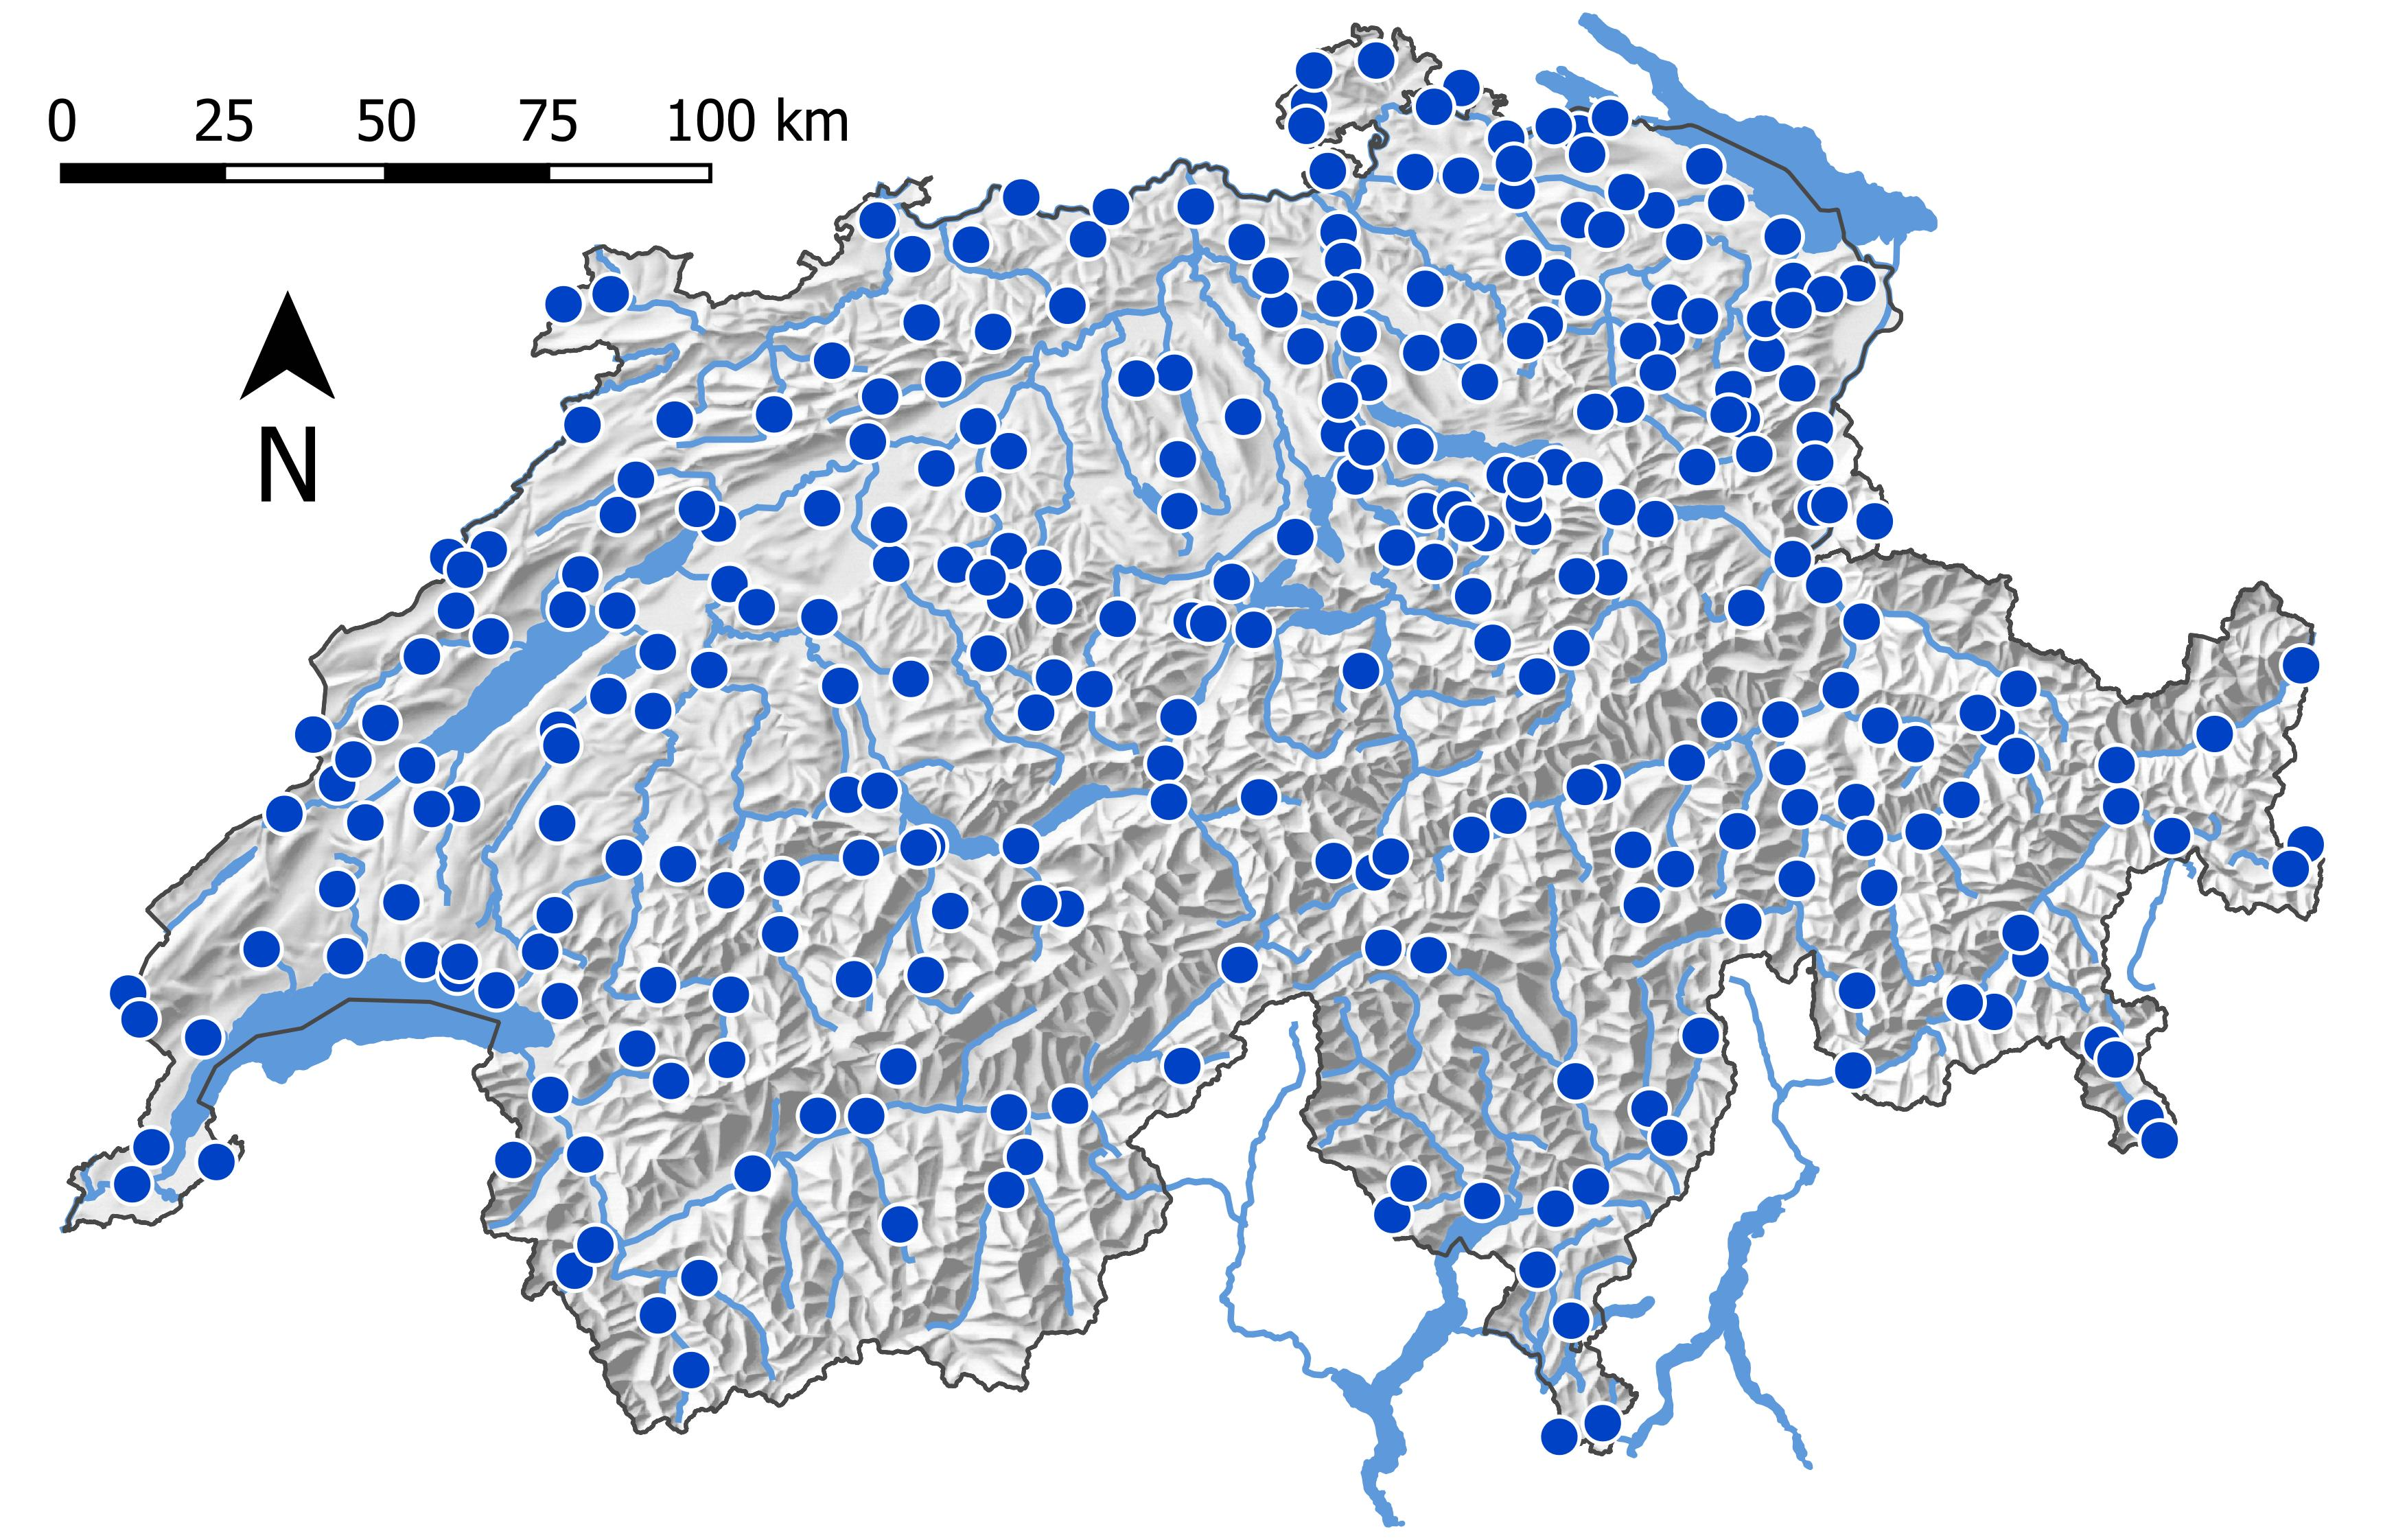
\includegraphics[width=70mm]{figures/map-stations.jpg}\\
	\caption{Map of the 301 precipitation stations with good data coverage of the period 1981--2010. Background map: \textcopyright\ SwissTopo.}
	\label{fig:stations}
\end{figure}


\subsection{Analog methods}

\begin{equation}
\label{eq:S1}
S1=100 \frac{\sum_{i} \vert \Delta\hat{z}_{i} - \Delta z_{i} \vert}{\sum_{i} \max\left\lbrace \vert \Delta\hat{z}_{i} \vert; \vert \Delta z_{i} \vert \right\rbrace }
% use \displaystyle to max sum sign larger
\end{equation}
where $\Delta \hat{z}_{i}$ is the geopotential height gradient between the \textit{i}-th pair of points for the target day, and $\Delta z_{i}$ is the corresponding observed geopotential height gradient for the candidate situation. The smaller the values S1 are, the more similar the pressure fields.


\begin{table*}[t]
	\caption{Analogue methods considered in the study, listed by increasing complexity. The analogy criterion is S1 for SLP and Z and RMSE for the other variables.}
	\small
	\begin{threeparttable}
	\begin{tabular}{llllll}
		\hline
		\headrow
		\thead{Method} & \thead{P0} & \thead{L1} & \thead{L2} & \thead{L3} & \thead{Reference} \\ 
		\hline 
		\multirow{2}{*}{\textbf{2Z}} & \multirow{2}{*}{PC} & Z1000@12h &&& \multirow{2}{*}{\citealp{Bontron2004}} \\
		&& Z500@24h &&& \\
		\hline 
		\multirow{4}{*}{\textbf{4Z}} & \multirow{4}{*}{PC} & Z1000@06h &&& \multirow{4}{*}{\citealp{Horton2018a}} \\
		&& Z1000@30h &&& \\
		&& Z700@24h &&& \\
		&& Z500@12h &&& \\
		\hline 
		\multirow{2}{*}{\textbf{2Z-2MI}} & \multirow{2}{*}{PC} & Z1000@12h & \multirow{2}{*}{MI850@12+24h} && \multirow{2}{*}{\citealp{Bontron2004}} \\
		&& Z500@24h &&& \\
		\hline 
		\multirow{4}{*}{\textbf{4Z-2MI}} & \multirow{4}{*}{PC} & Z1000@30h &&& \multirow{4}{*}{\citealp{Horton2018a}}\\
		&& Z850@12h & MI700@24h && \\
		&& Z700@24h & MI600@12h && \\
		&& Z400@12h &&& \\
		\hline 
		\multirow{2}{*}{\textbf{PT-2Z-4MI}} & T925@36h & Z1000@12h & MI925@12+24h && \multirow{2}{*}{\citealp{BenDaoud2016}} \\
		& T600@12h & Z500@24h & MI700@12+24h && \\
		\hline 
		\multirow{2}{*}{\textbf{PT-2Z-4W-4MI}} & T925@36h & Z1000@12h & \multirow{2}{*}{W850@06-24h} & MI925@12+24h & \multirow{2}{*}{\citealp{BenDaoud2016}} \\
		& T600@12h & Z500@24h && MI700@12+24h & \\
		\hline 
	\end{tabular} 

	\begin{tablenotes}
	\item P0, preselection (PC: $\pm 60$ days around the target date); L1, L2 and L3, subsequent levels of analogy.
	\item Z, geopotential height; T, air temperature; W, vertical velocity; MI, moisture index (product of the relative humidity at the given pressure level and the total water column).
	\end{tablenotes}
	\end{threeparttable}
	\label{table:methods}
\end{table*}


\section{Results}
\subsection{Impact on the skill}

\begin{figure}[bt]
    \centering
    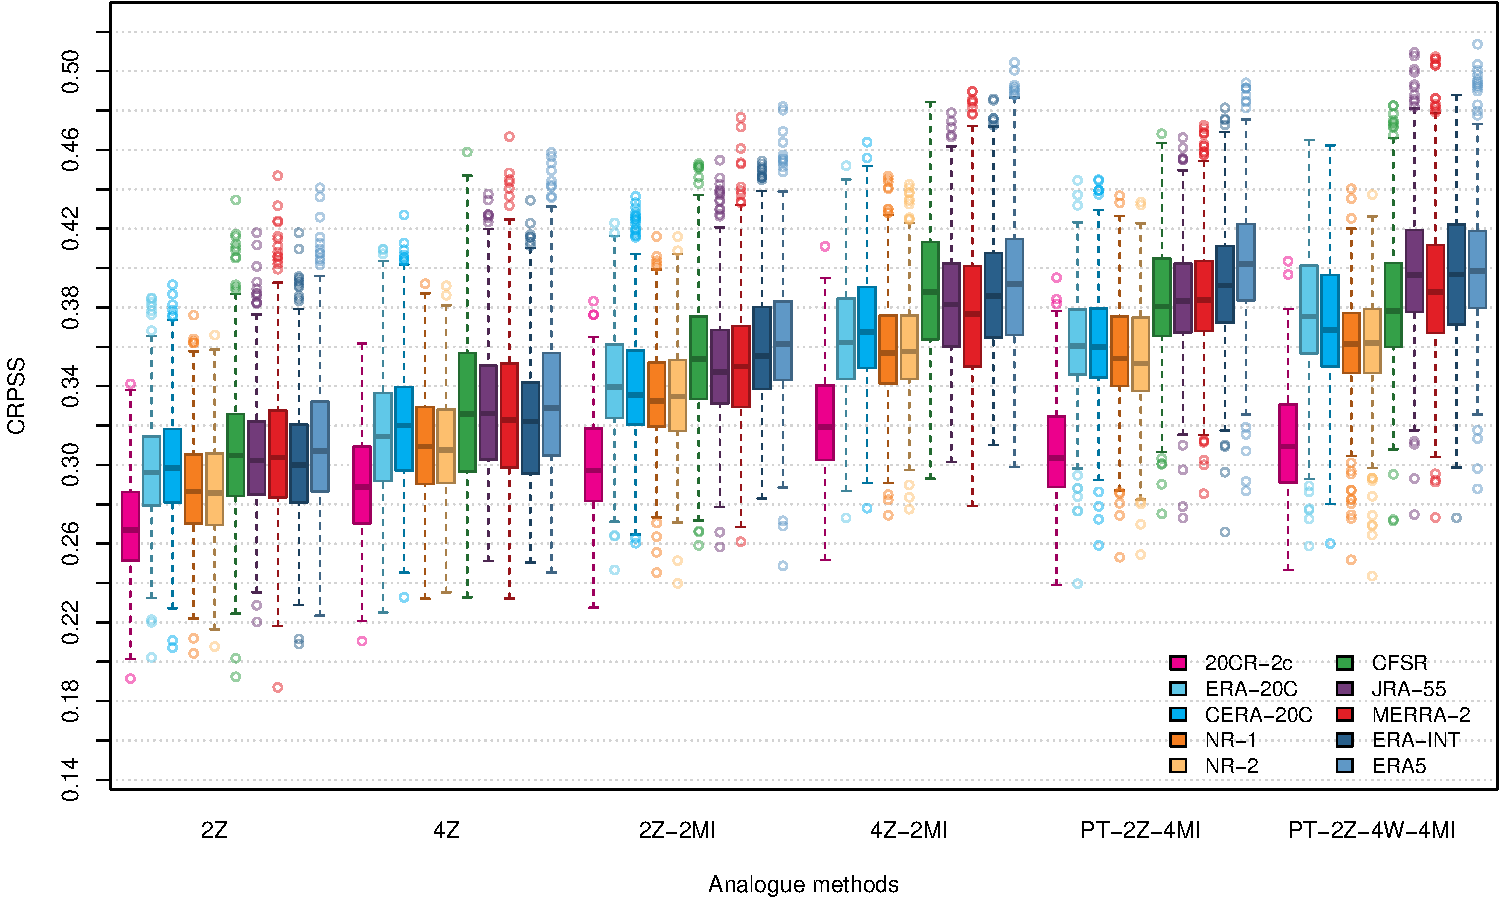
\includegraphics[width=\textwidth]{figures/boxplot-per-method.pdf}
    \caption{CRPSS for all stations, and for all considered AMs and reanalysis datasets on the VP. A higher CRPSS means better performance. The parameters of the AMs were calibrated for every station, every dataset, and every method. The boxes show the 25th, 50th, and 75th percentiles. The whiskers extend to the most extreme data point which is no more than 1.5 times the interquartile range.}
    \label{fig:comparison_values}
\end{figure}

\begin{figure}[bt]
    \centering
    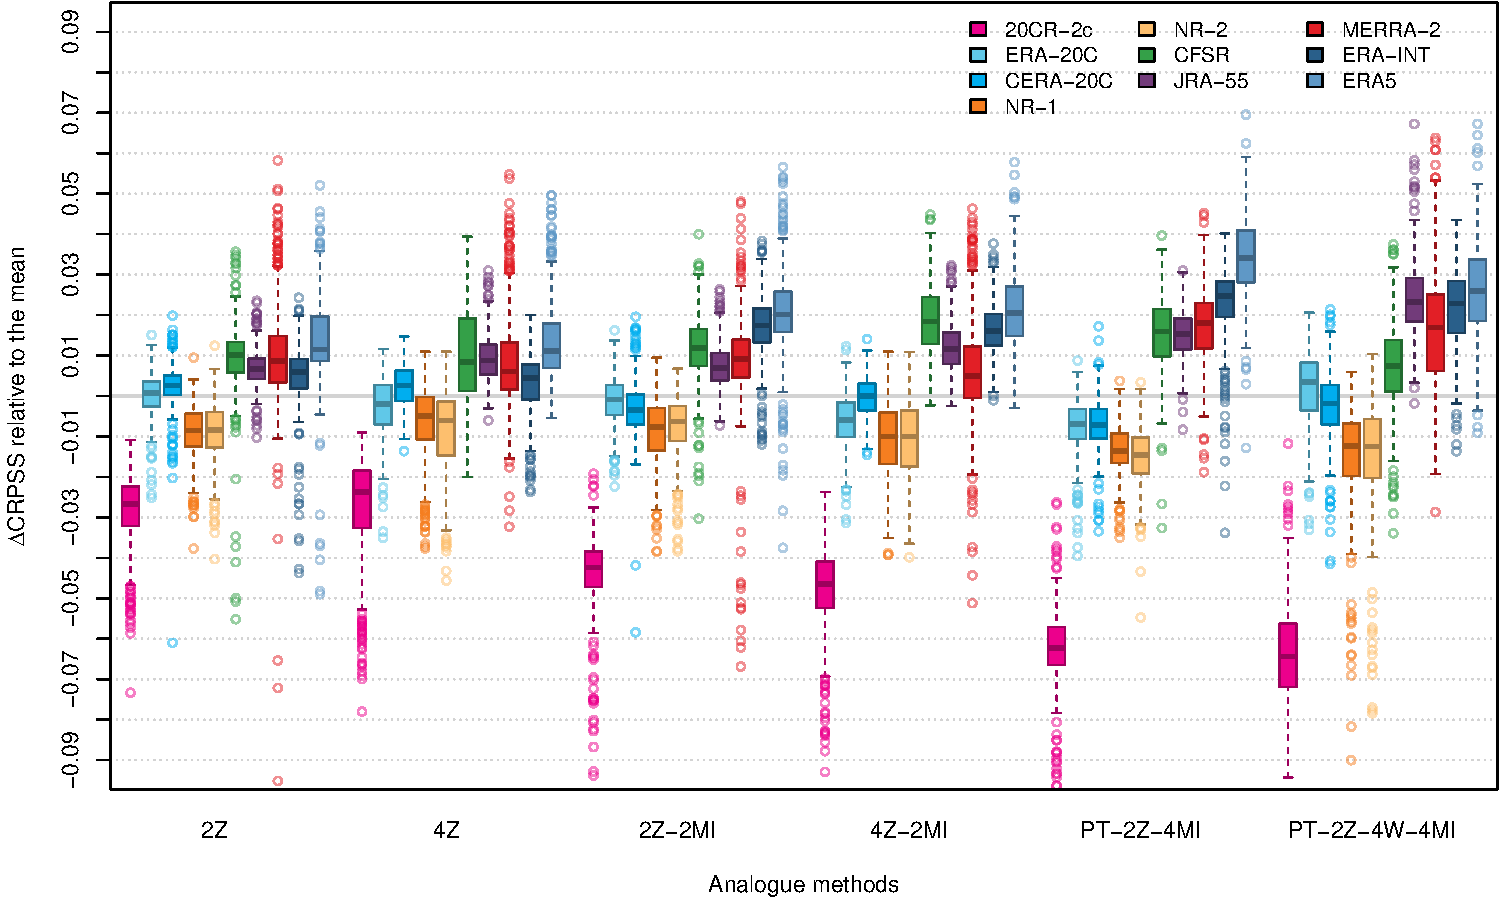
\includegraphics[width=\textwidth]{figures/boxplot-per-method-diff.pdf}
    \caption{Impact of the reanalysis dataset on performance, isolated by processing the improvement in CRPSS for one dataset compared to the mean performance on all datasets, per station and per method. Note that the methods cannot be compared here, only the datasets. Same conventions as Fig. 2.}
    \label{fig:comparison_relative}
\end{figure}

%TODO: coeff correl?
%TODO: biases

\subsection{High resolution and its pitfalls}


\begin{figure}[bt]
	\centering
	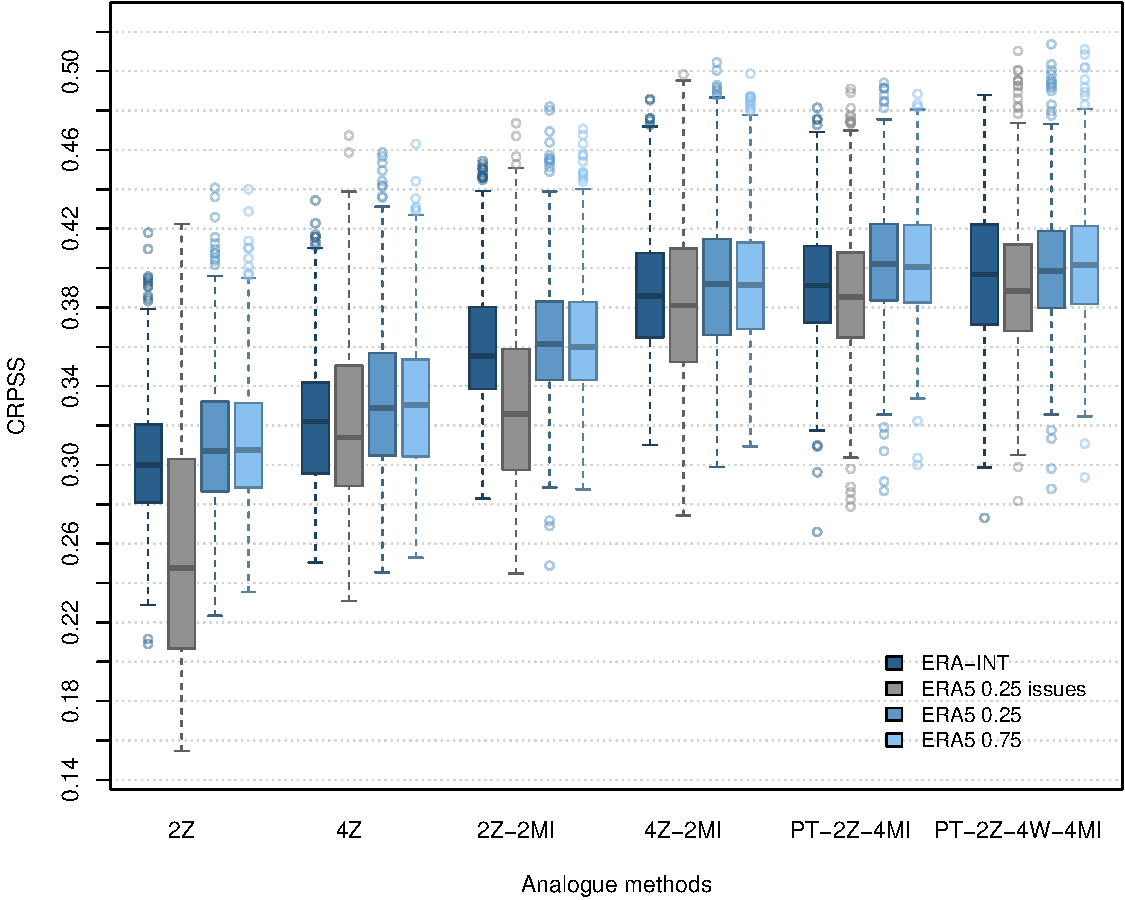
\includegraphics[width=80mm]{figures/boxplot-resol.pdf}
	\caption{....}
	\label{fig:resolution}
\end{figure}


\subsection{Shared analog dates}

\section{Conclusions}





\section{First Level Heading}
Please lay out your article using the section headings and example objects below, and remember to delete all help text prior to submitting your article to the journal.



\subsection{Second Level Heading}
If data, scripts or other artefacts used to generate the analyses presented in the article are available via a publicly available data repository, please include a reference to the location of the material within the article.


\subsection{Adding Citations and a References List}

Please use a \verb|.bib| file to store your references. When using Overleaf to prepare your manuscript, you can upload a \verb|.bib| file or import your Mendeley, CiteULike or Zotero library directly as a \verb|.bib| file\footnote{see \url{https://www.overleaf.com/blog/184}}. You can then cite entries from it, like this: \cite{lees2010theoretical}. Just remember to specify a bibliography style, as well as the filename of the \verb|.bib|.

You can find a video tutorial here to learn more about BibTeX: \url{https://www.overleaf.com/help/97-how-to-include-a-bibliography-using-bibtex}.

This template provides two options for the citation and reference list style: 
\begin{description}
\item[Numerical style] Use \verb|\documentclass[...,num-refs]{wiley-article}|
\item[Author-year style] Use \verb|\documentclass[...,alpha-refs]{wiley-article}|
\end{description}

\subsubsection{Third Level Heading}
Supporting information will be included with the published article. For submission any supporting information should be supplied as separate files but referred to in the text.

Appendices will be published after the references. For submission they should be supplied as separate files but referred to in the text.

\paragraph{Fourth Level Heading}
% Here are examples of quotes and epigraphs.
\begin{quote}
The significant problems we have cannot be solved at the same level of thinking with which we created them.\endnote{Albert Einstein said this.}
\end{quote}

\begin{epigraph}{Albert Einstein}
Anyone who has never made a mistake has never tried anything new.
\end{epigraph}

\subparagraph{Fifth level heading}
Measurements should be given in SI or SI-derived units.
Chemical substances should be referred to by the generic name only. Trade names should not be used. Drugs should be referred to by their generic names. If proprietary drugs have been used in the study, refer to these by their generic name, mentioning the proprietary name, and the name and location of the manufacturer, in parentheses.



\section*{acknowledgements}
Acknowledgements should include contributions from anyone who does not meet the criteria for authorship (for example, to recognize contributions from people who provided technical help, collation of data, writing assistance, acquisition of funding, or a department chairperson who provided general support), as well as any funding or other support information.

\section*{conflict of interest}
You may be asked to provide a conflict of interest statement during the submission process. Please check the journal's author guidelines for details on what to include in this section. Please ensure you liaise with all co-authors to confirm agreement with the final statement.

%\printendnotes

% Submissions are not required to reflect the precise reference formatting of the journal (use of italics, bold etc.), however it is important that all key elements of each reference are included.
\bibliography{references}


\graphicalabstract{example-image-1x1}{Please check the journal's author guildines for whether a graphical abstract, key points, new findings, or other items are required for display in the Table of Contents.}

\end{document}
